\documentclass[tikz,border=12pt]{standalone}
\usepackage[T1]{fontenc}
\usepackage{mathpazo}
\usepackage{amsmath,amssymb}
\usetikzlibrary{arrows.meta, positioning, calc, fit, decorations.pathreplacing}

\definecolor{stblue}{HTML}{7B97AD}
\definecolor{rwgold}{HTML}{B8995E}
\definecolor{sage}{HTML}{7A9A7E}
\definecolor{dkbrown}{HTML}{3D3530}
\definecolor{wmgray}{HTML}{7B7067}
\definecolor{cream}{HTML}{F9F6F0}
\definecolor{border}{HTML}{D4C9B8}
\definecolor{terracotta}{HTML}{C47A6A}
\definecolor{lavender}{HTML}{907EA0}

\begin{document}
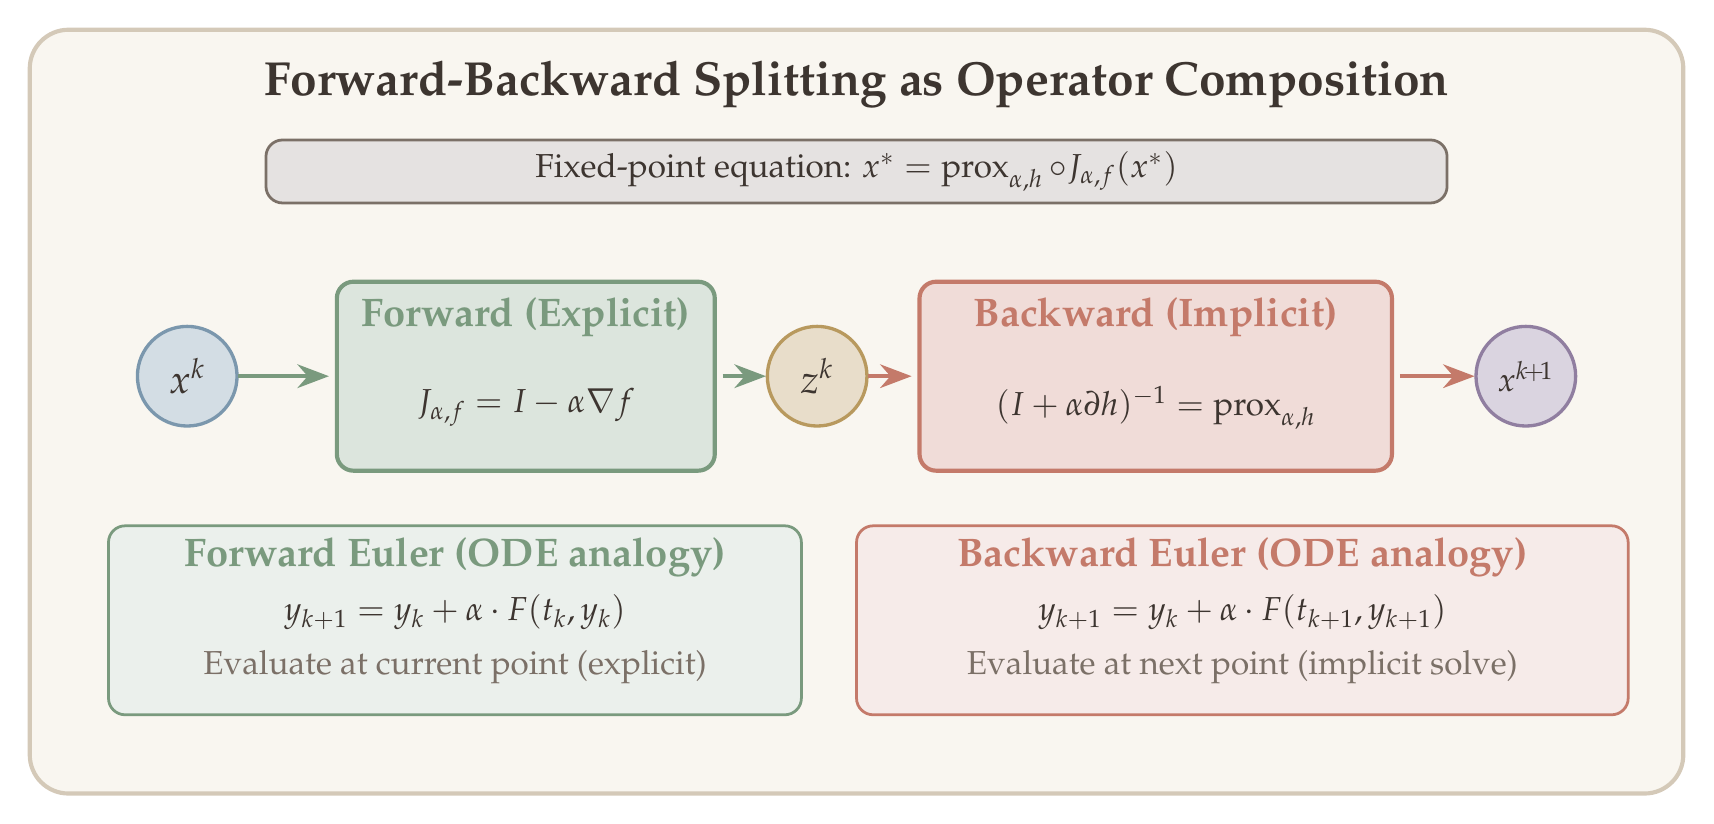
\begin{tikzpicture}[>={Stealth[length=4mm, width=3mm]}]

% Background
\fill[cream, rounded corners=14pt] (-0.5,-0.5) rectangle (20.5,9.2);
\draw[border, line width=1.5pt, rounded corners=14pt] (-0.5,-0.5) rectangle (20.5,9.2);

% Title
\node[text=dkbrown, font=\LARGE\bfseries] at (10,8.5) {Forward-Backward Splitting as Operator Composition};

% Optimality condition row
\fill[wmgray!20, rounded corners=6pt] (2.5,7.0) rectangle (17.5,7.8);
\draw[wmgray, line width=1pt, rounded corners=6pt] (2.5,7.0) rectangle (17.5,7.8);
\node[text=dkbrown, font=\large] at (10.0,7.4) {Fixed-point equation: $x^* = \operatorname{prox}_{\alpha,h} \circ J_{\alpha,f}(x^*)$};

% Node: x^k
\fill[stblue!33] (1.5,4.8) circle (18pt);
\draw[stblue, line width=1.2pt] (1.5,4.8) circle (18pt);
\node[text=dkbrown, font=\Large] at (1.5,4.8) {$x^k$};

% Forward step box
\fill[sage!26, rounded corners=6pt] (3.4,3.6) rectangle (8.2,6.0);
\draw[sage, line width=1.5pt, rounded corners=6pt] (3.4,3.6) rectangle (8.2,6.0);
\node[text=sage, font=\Large\bfseries] at (5.8,5.55) {Forward (Explicit)};
\node[text=dkbrown, font=\large] at (5.8,4.4) {$J_{\alpha,f} = I - \alpha\nabla f$};

% Arrow x^k -> Forward
\draw[sage, line width=1.5pt, ->] (2.15,4.8) -- (3.3,4.8);

% Node: z^k
\fill[rwgold!33] (9.5,4.8) circle (18pt);
\draw[rwgold, line width=1.2pt] (9.5,4.8) circle (18pt);
\node[text=dkbrown, font=\Large] at (9.5,4.8) {$z^k$};

% Arrow Forward -> z^k
\draw[sage, line width=1.5pt, ->] (8.3,4.8) -- (8.85,4.8);

% Backward step box
\fill[terracotta!26, rounded corners=6pt] (10.8,3.6) rectangle (16.8,6.0);
\draw[terracotta, line width=1.5pt, rounded corners=6pt] (10.8,3.6) rectangle (16.8,6.0);
\node[text=terracotta, font=\Large\bfseries] at (13.8,5.55) {Backward (Implicit)};
\node[text=dkbrown, font=\large] at (13.8,4.4) {$(I + \alpha\partial h)^{-1} = \operatorname{prox}_{\alpha,h}$};

% Arrow z^k -> Backward
\draw[terracotta, line width=1.5pt, ->] (10.15,4.8) -- (10.7,4.8);

% Node: x^{k+1}
\fill[lavender!33] (18.5,4.8) circle (18pt);
\draw[lavender, line width=1.2pt] (18.5,4.8) circle (18pt);
\node[text=dkbrown, font=\large] at (18.5,4.8) {$x^{k\!+\!1}$};

% Arrow Backward -> x^{k+1}
\draw[terracotta, line width=1.5pt, ->] (16.9,4.8) -- (17.85,4.8);

% Bottom: ODE parallel
\fill[sage!15, rounded corners=6pt] (0.5,0.5) rectangle (9.3,2.9);
\draw[sage, line width=1pt, rounded corners=6pt] (0.5,0.5) rectangle (9.3,2.9);
\node[text=sage, font=\Large\bfseries] at (4.9,2.5) {Forward Euler (ODE analogy)};
\node[text=dkbrown, font=\large] at (4.9,1.8) {$y_{k+1} = y_k + \alpha \cdot F(t_k, y_k)$};
\node[text=wmgray, font=\large] at (4.9,1.1) {Evaluate at current point (explicit)};

\fill[terracotta!15, rounded corners=6pt] (10.0,0.5) rectangle (19.8,2.9);
\draw[terracotta, line width=1pt, rounded corners=6pt] (10.0,0.5) rectangle (19.8,2.9);
\node[text=terracotta, font=\Large\bfseries] at (14.9,2.5) {Backward Euler (ODE analogy)};
\node[text=dkbrown, font=\large] at (14.9,1.8) {$y_{k+1} = y_k + \alpha \cdot F(t_{k+1}, y_{k+1})$};
\node[text=wmgray, font=\large] at (14.9,1.1) {Evaluate at next point (implicit solve)};

\end{tikzpicture}
\end{document}
